%% Exemplo de utilizacao do estilo de formatacao normas-utf-tex (http://normas-utf-tex.sourceforge.net)
%% dúvidas acessar o site acima
%%
%%
%% Autores: (200?-2011) Hugo Vieira Neto (hvieir@utfpr.edu.br)
%%          (200?-2011) Diogo Rosa Kuiaski (diogo.kuiaski@gmail.com)
%%          (2011-2017) Marcos Talau <talau@users.sourceforge.net>
%% Colaborador:
%%          (2011) César M. Vargas Benitez <cesarvargasb@gmail.com>

%%
%% IMPORTANTE: O texto está escrito com acentuação antiga, atualmente você
%%             pode escrever acentos sem precisar de códigos para tal.
%%

\documentclass[openright]{normas-utf-tex} %openright = o capitulo comeca sempre em paginas impares
%\documentclass[oneside]{normas-utf-tex} %oneside = para dissertacoes com numero de paginas menor que 100 (apenas frente da folha) 

% force A4 paper format
\special{papersize=210mm,297mm}

\usepackage[alf,abnt-emphasize=bf,bibjustif,recuo=0cm, abnt-etal-cite=2, abnt-etal-list=99]{abntcite} %configuracao correta das referencias bibliograficas.

\usepackage[utf8]{inputenc} % pacote para acentuacao direta
\usepackage{amsmath,amsfonts,amssymb} % pacote matematico
\usepackage{graphicx} % pacote grafico
\usepackage[final]{pdfpages} % adicao da ata
\usepackage{float}

%Podem utilizar GEOMETRY{...} para realizar pequenos ajustes das margens. Onde, left=esquerda, right=direita, top=superior, bottom=inferior. P.ex.:
%\geometry{left=3.0cm,right=1.5cm,top=4cm,bottom=1cm} 

% ---------- Preambulo ----------
\instituicao{Federal University of Technology - Paraná} % nome da instituicao
\programa{Department of Electronics} % nome do programa
\area{Electronics Engineering} % [Engenharia Biomedica] ou [Informatica Industrial] ou [Telematica]

\documento{Undergraduate Thesis}
\nivel{Bacharelado} % [Mestrado] ou [Doutorado]
\titulacao{Bacharel} % [Mestre] ou [Doutor]

\titulo{{zCart: A smart cart prototype}} % titulo do trabalho em portugues
\title{\MakeUppercase{zCart: A smart cart prototype}} % titulo do trabalho em ingles

\autor{Flávio Shigueo Miamoto} % autor do trabalho
\autordois{João Pedro Zanlorensi Cardoso} % autor do trabalho
\cita{MIAMOTO, Flavio; ZANLORENSI, Joao Pedro} % sobrenome (maiusculas), nome do autor do trabalho

\palavraschave{Artificial Inteligenge, Deep Learning, Smart Devices, Internet of Things} 

\comentario{\UTFPRdocumentodata\ presented to the \UTFPRprogramadata\ of the \ABNTinstituicaodata\ as a partial requisite for obtaining the Bachelor in Electronics Engineering degree}

\orientador{André Eugênio Lazaretti, Ph.D}

\local{Curitiba} % cidade
\data{\the\year} % ano automatico

% desativa hifenizacao mantendo o texto justificado.
% thanks to Emilio C. G. Wille
\tolerance=1
\emergencystretch=\maxdimen
\hyphenpenalty=10000
\hbadness=10000
\sloppy

%---------- Inicio do Documento ----------
\begin{document}

\capa % geracao automatica da capa
\folhaderosto % geracao automatica da folha de rosto

% dedicatoria
\begin{dedicatoria}
    To all our families and their unconditional support
\end{dedicatoria}

% agradecimentos (opcional)
\begin{agradecimentos}
    We thank everyone that helped
\end{agradecimentos}

% epigrafe (opcional)
\begin{epigrafe}
 If have seen further it is by standing on the shoulders of giants.  \\
- Sir Isaac Newton
\end{epigrafe}

%abstract
\begin{abstract}
Abstract text (maximum of 500 words).
\end{abstract}

% listas (opcionais, mas recomenda-se a partir de 5 elementos)
\listadefiguras % geracao automatica da lista de figuras
\listadetabelas % geracao automatica da lista de tabelas
% \listadequadros % adivinhe :)
\listadesiglas % geracao automatica da lista de siglas
\listadesimbolos % geracao automatica da lista de simbolos

% sumario
\sumario % geracao automatica do sumario


%---------- Inicio do Texto ----------
% recomenda-se a escrita de cada capitulo em um arquivo texto separado (exemplo: intro.tex, fund.tex, exper.tex, concl.tex, etc.) e a posterior inclusao dos mesmos no mestre do documento utilizando o comando \input{}, da seguinte forma:
%\input{intro.tex}
%\input{fund.tex}
%\input{exper.tex}
%\input{concl.tex}

\setcounter{page}{12}

\chapter{Introduction}

With the advancement of the high speed mobile networks and smartphone penetration,
customer demands are on an ever increasing trajectory for more personalized
and digital experiences. In that regard, companies worldwide are fighting for customer
attention in the digital era by developing products and services that bring state-of-the-art technologies
to the masses in the so called smart devices and systems \cite{Shafique2020}.

As an example of such advancements, smart speakers such as the Amazon Echo \cite{GaoPanWangChen2018} include the latest and greatest
in terms of Natural Language Processing and Deep Learning \cite{Young2018}, allowing customers to interact with the product in an conversational manner
that was considered to be science fiction material until a couple of years ago.

\begin{figure}[!htb]
	\centering
	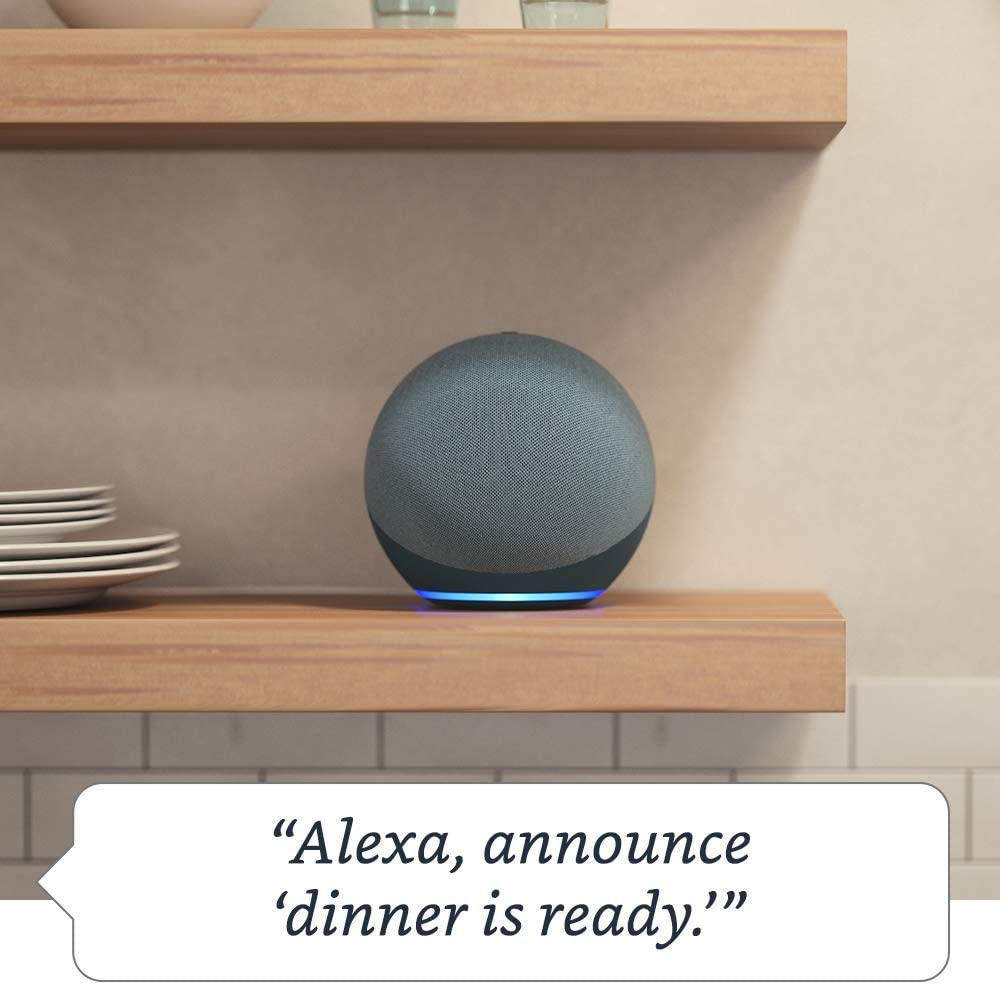
\includegraphics[width=0.4\textwidth]{./images/echodot4.jpg} % <- formatos PNG, JPG e PDF
	\caption[Amazon Echo 4th Generation smart speaker promotional material]{Amazon Echo 4th Gen Smart Speaker promotional material}
    \fonte{Amazon (2022)}
	\label{fig:echodot4}
\end{figure}

\begin{quote}
    \textit{This device is a gem! When I’m busy in the kitchen, for example, and can’t get
    to a computer to find info or music to play, Alexa would be there to listen
    and do what I ask.} \\
    Customer review from \cite{GaoPanWangChen2018}
\end{quote}

Alongside the devices themselves, entirely new markets have emerged such as the third-party software extensions
called \textit{Alexa Skills} \cite{Alexa2022}.

These skills function much like mobile phone apps, extending and enhancing the functionality of the device, and
can be sold to users.

Developers are can then leverage the highly advanced machine learning models - which can be notoriously expensive to develop 
and maintain \cite{Phdata2021} - through \sigla{API}{Application Programming Interface}s and focus exclusively on their application logic.

\begin{figure}[htb!]
	\centering
	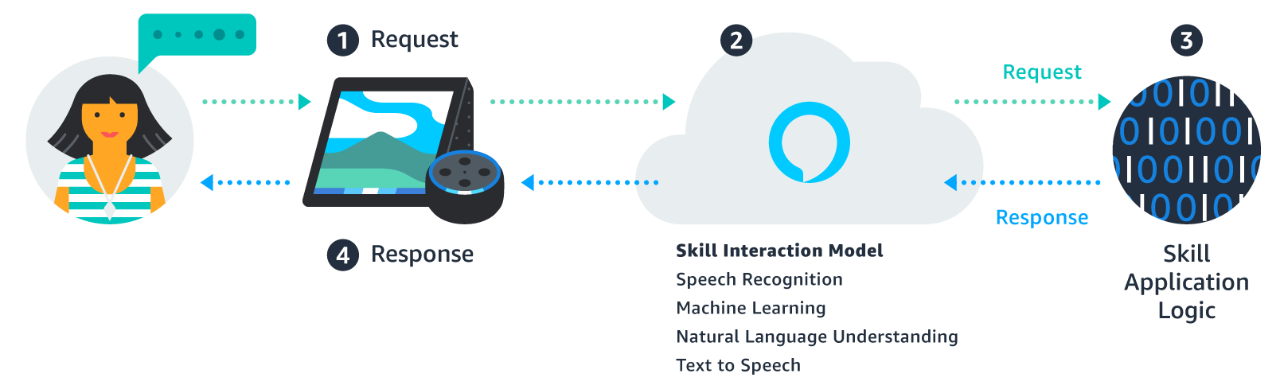
\includegraphics[width=0.9\textwidth]{./images/skills.png} % <- formatos PNG, JPG e PDF
	\caption[Diagram showing the steps of an interaction with an Alexa Skill]{Diagram showing the steps of an interaction with an Alexa Skill}
    \fonte{\cite{Alexa2022}}
	\label{fig:alexaskill}
\end{figure}

More impressively, such technological advancements have been able to reach a considerable amount of households in
a short period in developed countries like the United States, a display of the power of the economy of scale and how
an extensible ecosystem can boost sales.

\begin{figure}[H]
	\centering
	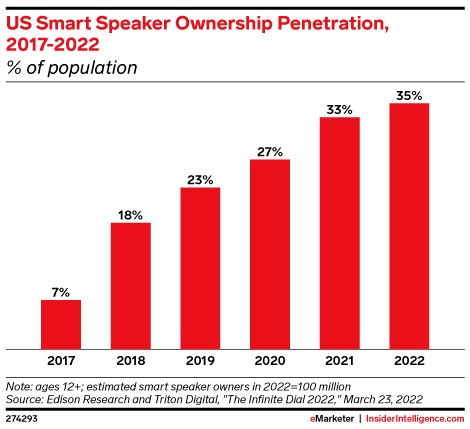
\includegraphics[width=0.6\textwidth]{./images/smartspeaker.png} % <- formatos PNG, JPG e PDF
	\caption[US Smart Speaker Penetration from 2017 to 2022]{US Smart Speaker Penetration from 2017 to 2022}
    \fonte{\cite{InsiderIntelligence2022}}
	\label{fig:smartspeaker}
\end{figure}

On developing countries, such as Brazil, these innovations tend to have delayed
arrivals due to historical economic barriers but the potential customer base
has attracted big tech companies and their economic power, shortening the
delay.

\begin{figure}[h!]
	\centering
	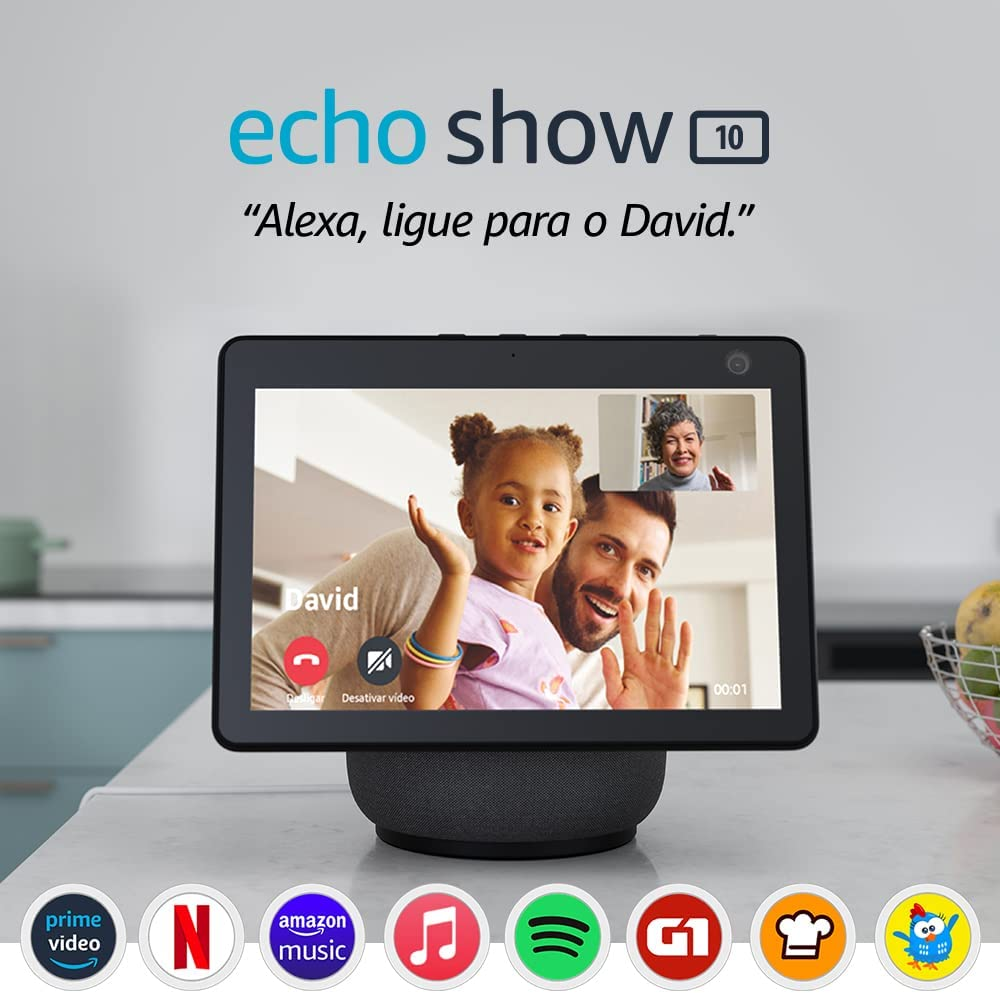
\includegraphics[width=0.4\textwidth]{./images/alexabr.jpg} % <- formatos PNG, JPG e PDF
	\caption[Localized promotional material for the Echo Show 10 targeting Brazilian customers]{Localized promotional material for the Echo Show 10 targeting Brazilian customers}
    \fonte{Amazon (2022)}
    \label{fig:alexabr}
\end{figure}

According to the research company IDC Brasil, the home automation market - in
which smart speakers are included - would have reached US\$ 298 million on
2021.

Although these advancements might seem entirely beneficial at first, countless
challenges have been found regarding privacy, ethical handling of personal
customer data and overall negative experiences caused by increased
dependencies, e.g what happens when you lose internet connection?

These discussions are of the utter most importance given our current scenario
and have been brought up by recent literature \cite{Echoes2022,He2019}
but will be out of the scope of our work.

\section{Motivation}

Even with all of these innovations impacting customer behaviors day by day, one
important aspect of consumer life still hasn't had any significant changes in
the last couple of years on the brazilian market: \textbf{grocery shopping on
physical stores}.

According to \sigla{ABRAS}{Associação Brasileira de Supermercados} - the
Brazilian Supermarket Association - the grocery retail sector has reached an
impressive total revenue of \textbf{R\$ 611 billion} - roughly US\$ 117 billion on
October 2022 - in 2021, making up 7.03\% of the national \sigla{GDP}{Gross
Domestic Product}. About \textbf{28 million} customers visit of the more than
\textbf{92,000} stores countrywide on a daily basis \cite{Abras2022}.

In the recent pandemic scenario, innovations such as the adoption of e-commerce platforms and
self-checkout solutions had their adoption increased in 2020 but 2021 showed that consumers have
mostly shifted back to their pre-pandemic behavior, favoring physical retail stores \cite{Kantar2022}.

But in such an economic relevant market and with all the technological
advancement we've been seing, most of the physical retail customers still
report pain points related to visiting a store. In a survey conducted in 2019,
Capgemini has found out five key problems \cite{Capgemini2020}:

\begin{enumerate}
        \item Long queues for payment checkout
        \item Out of stock products
        \item Difficulties in locating products in the store
        \item Not being able to find a store associate to help me
        \item Lack of product information when I select products
\end{enumerate}

\begin{figure}[H]
	\centering
	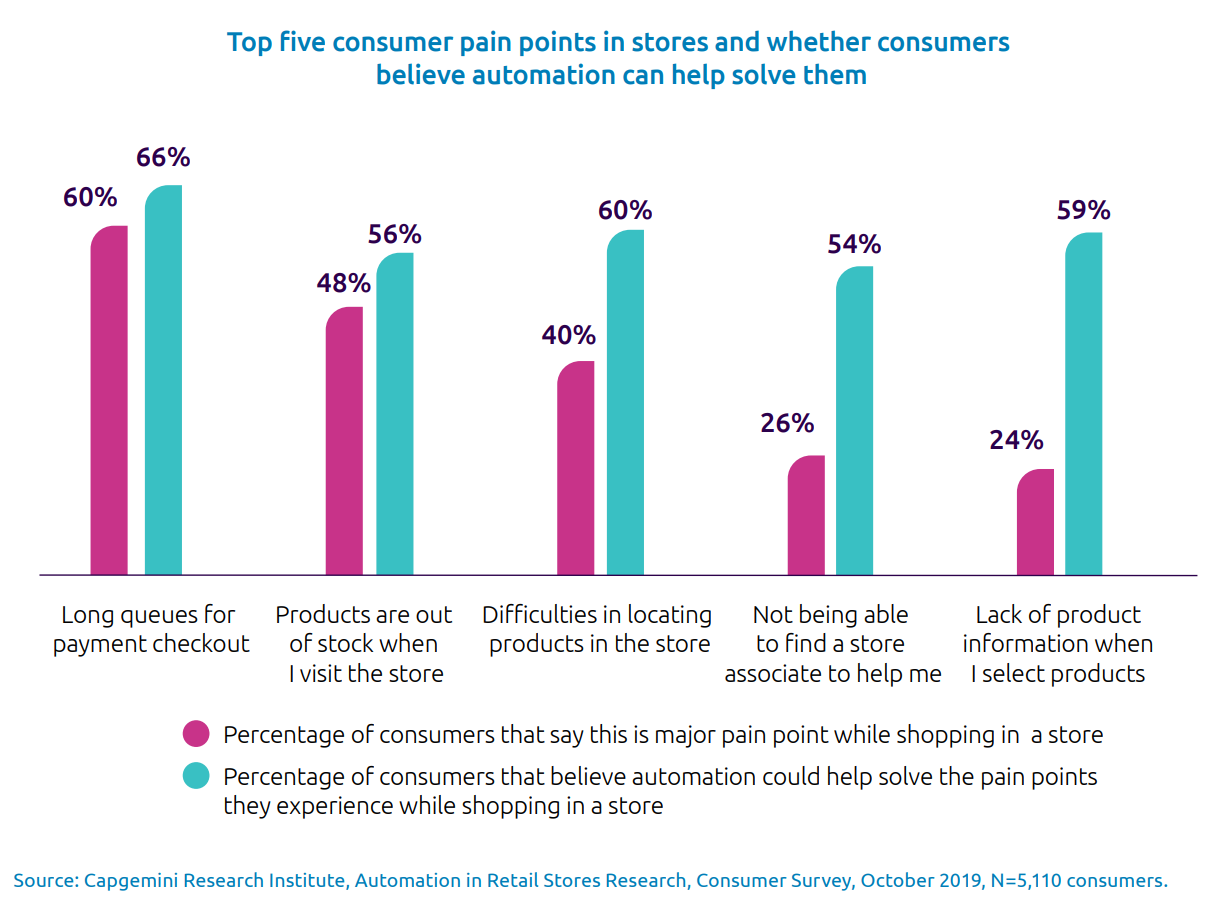
\includegraphics[width=0.8\textwidth]{./images/painpoints.png}
    \caption[Top five customer pain points in retail stores]{Top five customer pain points in retail stores}
    \fonte{\cite{Capgemini2020}}
    \label{fig:capgemini}
\end{figure}

More interestingly, Figure \ref{fig:capgemini} shows that at least half of the
survey respondents believe that all of the five pain points can be solved through
\textbf{automation}.

It is in this scenario of customer pain and enormous market potential that this
thesis will explore a technological solution to improve customer experience,
namely the \textbf{smart shopping cart}.

\section{Current scenario}

In this next section, we'll explore some of the existing solutions and how they
try to improve customer experience and increase the retailer's revenue.

\subsection{Caper Cart}

Developed by the Caper\footnote{https://caper.ai} company, the Caper Cart was the worlds's first AI-powered smart cart \cite{Caper2020}

The first version was launched in 2017 and offered grocers the
great advantage of not requiring any infrastructure overhaul for deployment.

\begin{figure}[H]
	\centering
	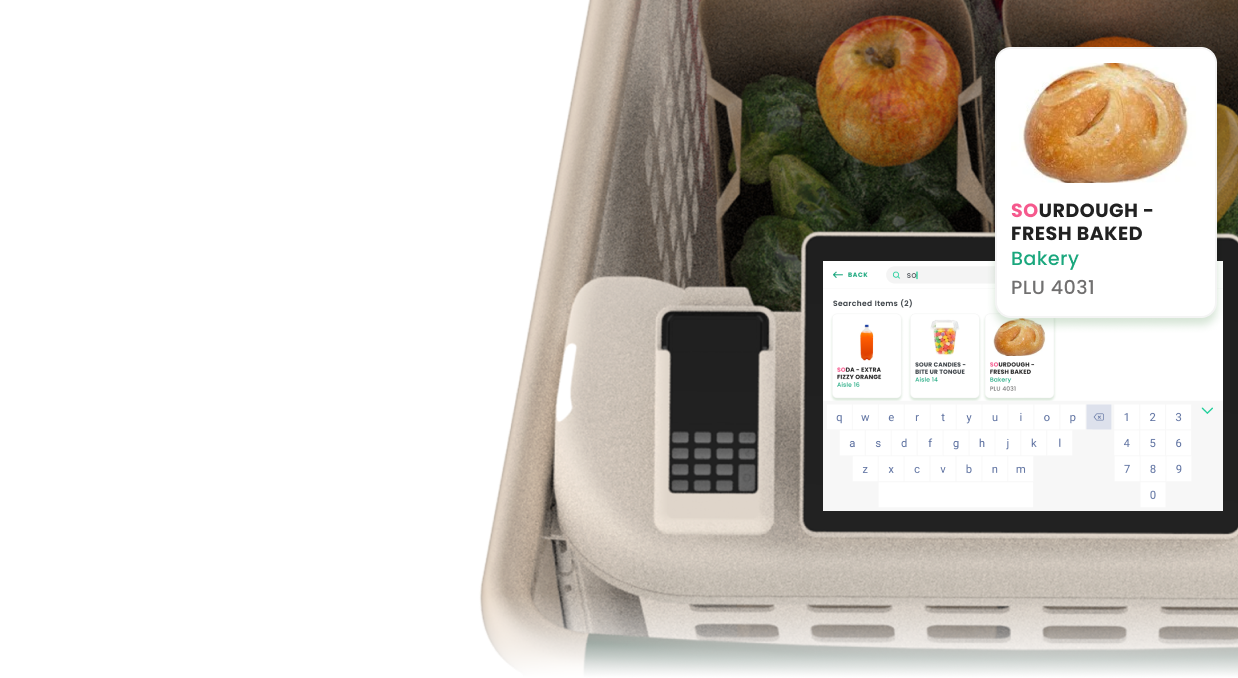
\includegraphics[width=0.7\textwidth]{./images/capercartui.png}
	\caption[Caper Cart user interface]{Caper Cart user interface}
    \fonte{Caper (2020)}
	\label{fig:caperui}
\end{figure}

\begin{figure}[H]
	\centering
	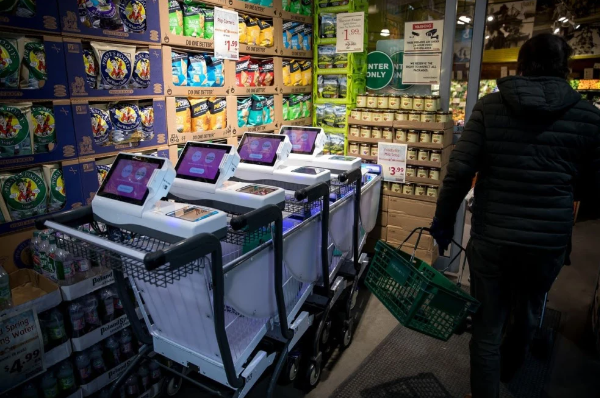
\includegraphics[width=0.7\textwidth]{./images/caper.png}
	\caption[Caper Cart at a retail store]{Caper Cart at a retail store}
    \fonte{Caper (2020)}
	\label{fig:caperatretail}
\end{figure}

For customers, it offered visual product recognition and a payment terminal,
allowing customers to avoid the dreaded queues by the end of their shopping.
Additionally, customers were able to search products, get discounts and locate
items more easily with the help of the user interface provided by the cart.

Although Caper does not publicize the cost of each cart, it is estimate that each unit costs between
\textbf{US\$ 5,000 and 10,000} \cite{TWP2021}.

Acquired by Instacart\footnote{https://instacart.com} in 2021 for US\$ 350 million, Caper is developing in 2022 the 
third version of its Smart Shopping Cart, advertising an increase in \textbf{65\% in the basket
volume} and a \textbf{10 month} breakeven.

\begin{figure}[H]
	\centering
	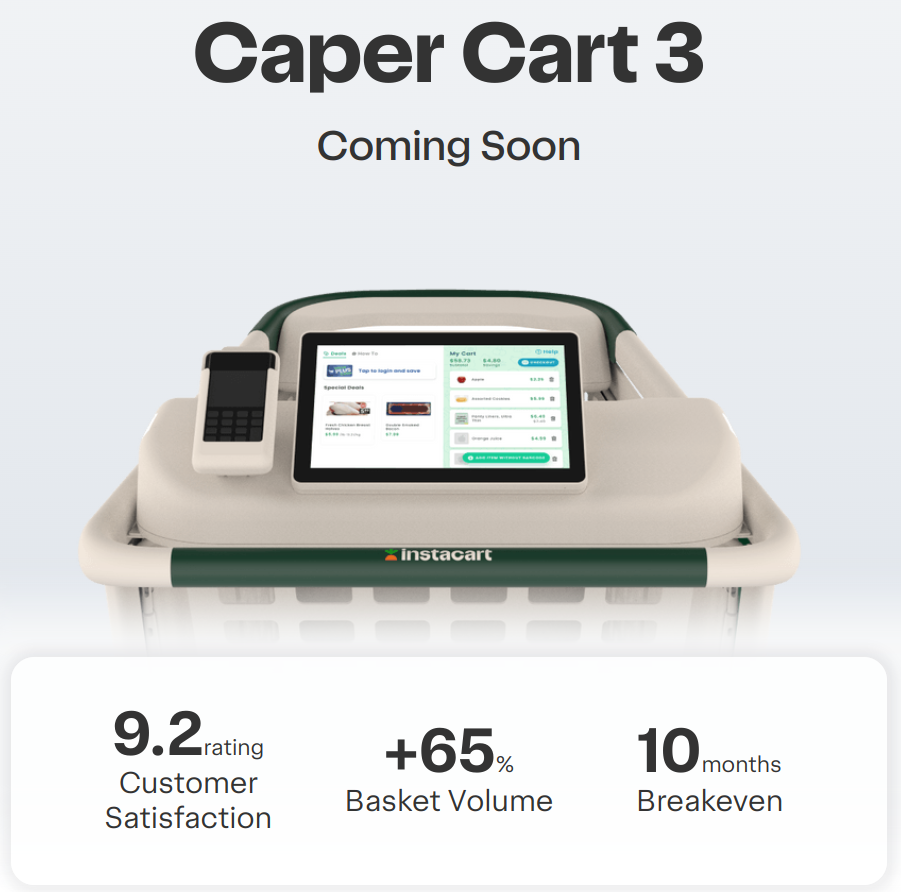
\includegraphics[width=0.7\textwidth]{./images/capercart3.png}
	\caption[Caper Cart 3 promotional material]{Caper Cart 3 promotional material}
    \fonte{Caper (2022)}
	\label{fig:nextop}
\end{figure}


\subsection{Amazon Dash Cart}

Available at the Amazon Fresh\footnote{https://www.amazon.com/fmc/m/30003175?almBrandId=QW1hem9uIEZyZXNo} retail chain, the
Amazon Dash Cart.

According to Amazon, it uses computer vision and sensors to allow customers to
simply add items to their cart which already accounts all the items and
subtotal. By the end of their item selection, customers can check-out
automatically without having to go through queues, solving the biggest customer
pain point pointed out by Capgemini.

\begin{quote}
\textit{Looking to make grocery trips quicker? With the Amazon Dash Cart you can skip the checkout line and roll out to your car when you are done.}

\textit{The Dash cart uses a combination of computer vision algorithms and sensor fusion to help identify items placed in the cart - simply grab an item, scan it on one of the Dash Cart cameras, and place it in the cart like you normally would.}
\\
Amazon (2022)
\end{quote}R

\begin{figure}[H]
	\centering
	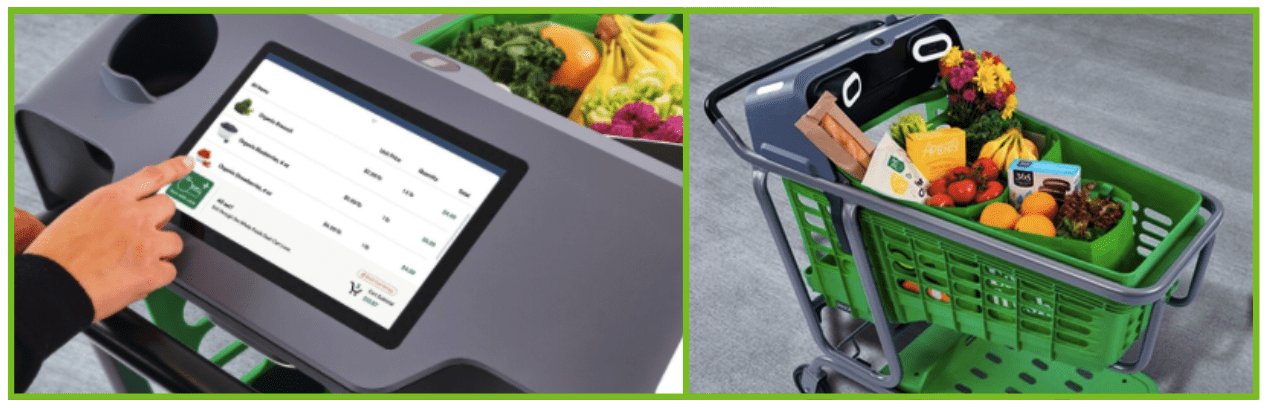
\includegraphics[width=0.8\textwidth]{./images/dashcart.png}
    \caption[Amazon Dash Cart]{Amazon Dash Cart}
    \fonte{Amazon (2022)}
    \label{fig:dashcart}
\end{figure}

Additionally, the user interface provided by the Cart allows customers to search for item location and see more information
about them, improving the customer experience.

One of its quircks is that it requires the download and usage of an mobile phone app for using the cart, in contrast
to Caper's Cart.

As of October 2022, the Amazon Dash Cart is exclusively available at the Amazon
Fresh chain and therefore no commercial information regarding cost per unit is
available.

\subsection{Nextop}

Founded in 1997, Nextop\footnote{https://nextop.com.br} is a Brazilian company
that develops products with a focus on the grocer market with an emphasis on
loss prevention.

According to the company, the Smart Cart Nextop is the first smart cart
deployed in Brazil and Latin America and was initially rolled out to the Enxuto
supermarket chain, present in the São Paulo state, on 2022 \cite{Paraiba2022}.

\begin{figure}[H]
	\centering
	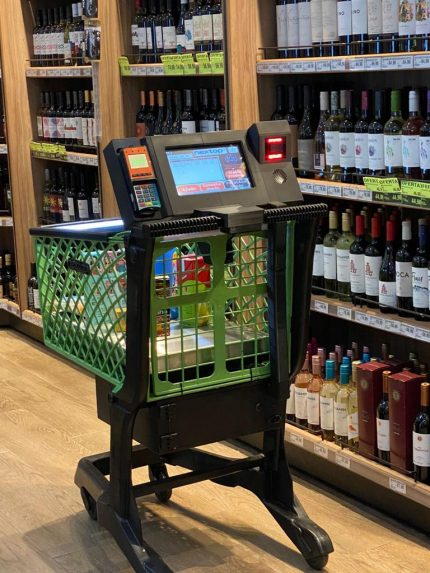
\includegraphics[width=0.4\textwidth]{./images/nextop.jpeg}
	\caption[Smart Cart Nextop® deployed to a Brazilian supermarket]{Smart Cart Nextop® deployed to a Brazilian supermarket}
    \fonte{Nextop (2022)}
	\label{fig:nextop}
\end{figure}

Differently than the carts developed by Amazon and Caper, Nextop's cart
requires customers to first scan the product using the integrate bar code
reader, as shown on Figure \ref{fig:nextopui}. This way, the product advertises
\textit{triple validation} using the cameras, sensors and the barcode scanner \cite{Nextop2022}.

\begin{figure}[H]
	\centering
	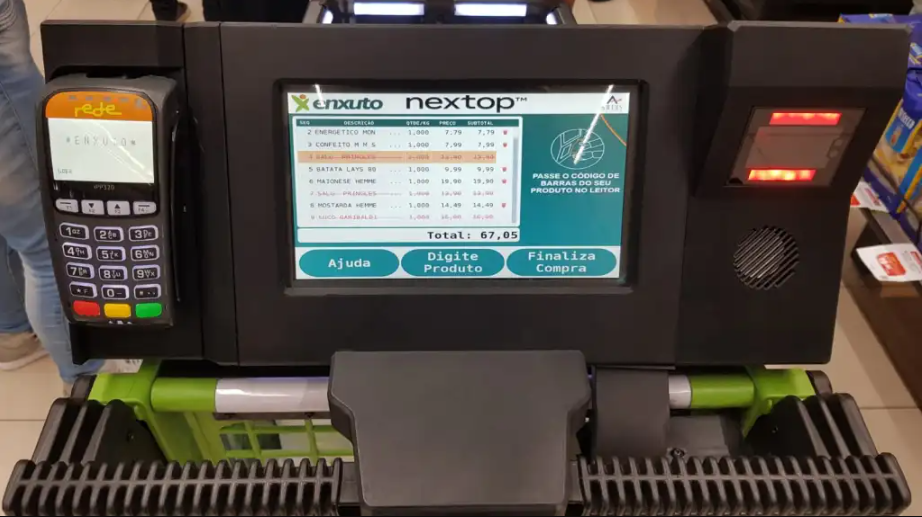
\includegraphics[width=0.9\textwidth]{./images/nextop2.png}
    \caption[Smart Cart Nextop® user interface with a payment terminal]{Smart Cart Nextop® user interface with a payment terminal}
    \fonte{\cite{Paraiba2022}}
	\label{fig:nextopui}
\end{figure}

Although it pleases grocers with the improved loss prevention, the usage of the barcode scanner creates in our opinion a worse
end customer experience, becoming a sort of \textit{mobile checkout station}.

\begin{figure}[H]
	\centering
	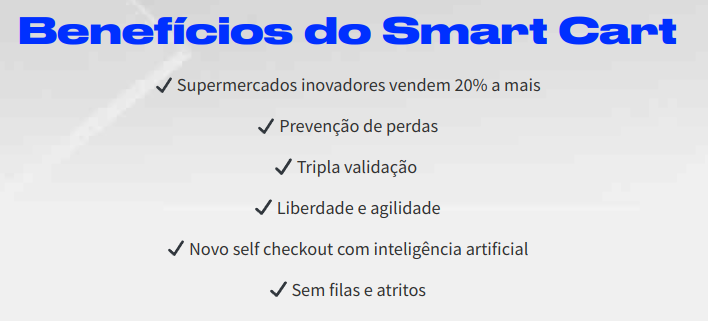
\includegraphics[width=0.9\textwidth]{./images/nextoppromo.png}
    \caption[Smart Cart Nextop® promotinal material targetting supermarket owners]{Smart Cart Nextop® promotinal material targetting supermarket owners}
    \fonte{\cite{Nextop2022}}
	\label{fig:nextopui}
\end{figure}

Besides offering the improve shopping experience by not having to go through queues by the end of the trip, the product advertises increased sales
as a result of the innovative approach and also allows a deeper understanding of the customer journey by collecting analytical data \cite{Paraiba2022}.

\begin{quote}
\textit{We are offering our customers an innovative and unique shopping experience within Enxuto}

\textit{With the smart cart, we broke through this barrier and managed to monitor the
entire customer's purchase circuit in the physical store. We have moved
from the identified ticket era to the end-to-end identified journey}

    Bruno Bragancini Junior, \sigla{CEO}{Chief Executive Officer} of the Enxuto Group \cite{Paraiba2022}
\end{quote}


This goes in line with the
company's know how on loss prevention which appeared to be an important aspect
of the product for the target Brazilian customer base.


According to Nextop's CEO, Juliano Camargo, the company has already invested \textbf{R\$ 8.5 million} - about US\$ 1.63 million on October 2022 - and \textbf{4 and half years}
of research and development.

Each Smart Cart is estimated to cost around \textbf{R\$ 120,000  or around US\$ 23,020} on October 2022 \cite{Paraiba2022}.

\section{Expected outcomes}

After presenting the problem domain and the current solutions, in this section we discuss the expected
outcomes of this work, mainly:

\textit{Develop a prototype of a smart shopping cart, including a mechanical assembly using with computer vision for object recognition
and an interactive user interface}

In a more granular level, these outcomes are also expected:

\begin{itemize}
    \item Collect a product dataset for traning a deep learning model
    \item Train a Deep Learning model capable of detecting target products
	\item Learn the practical challenges of developing a Deep Learning based product
    \item Understand the economic viability of such a project in the Brazilian context
\end{itemize}

Given our time and financial constraints, it is expected that the final results will yield
a solution with unsolved challenges, but a functional version is expected.

\chapter{Theoretical Background}

In this section, we'll define in greater detail some most relevant techniques
used in the development of our prototype.

This section can be skipped for readers with familiarity on the topics discussed

\section{Deep Learning}

\section{Neural Networks}

\section{Strain Gauge}

\section{Load Cell}

\section{HX711}

The HX711 is a 24-bit analog-to-digital converter (\sigla{ADC}{Analog-to-Digital Converter})
capable of outputting data in a Serial Interface (ADD CITATION).

It has two channels for analog input with channel A having programable gains of 128 or 64.

For power supply, it can be used with both 3.3\simbolo{V}{Volts} and 5 V standard digital voltages.

One of its advantages is is that there's no need to program internal registers, all
controls to the chip are through its pins.

\begin{figure}[H]
	\centering
	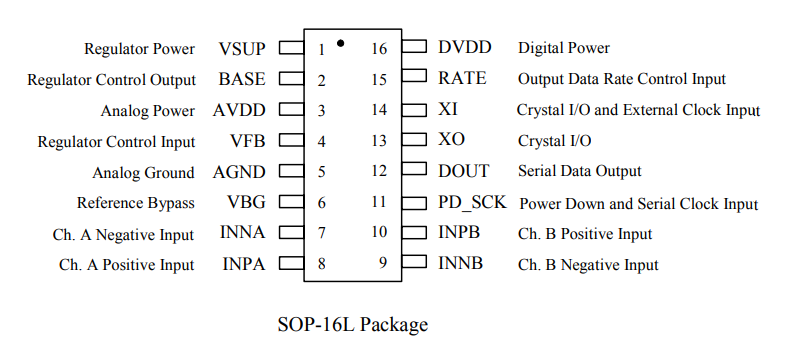
\includegraphics[width=1\textwidth]{./images/hx711-pinout.png}
	\caption[HX711 Pinout for the SOP-16L package]{HX711 Pinout for the SOP-16L package}
    \fonte{\cite{Avia2022}}
	\label{fig:architecture}
\end{figure}

\section{RESTful APIs}

\section{SQLite}

\section{Websockets}

\chapter{Development}
\label{chap:desenv}

\section{Design}

As a first step in developing our prototype, a set of
responsibilities was established to guide the high level design and is listed below:

\begin{enumerate}
    \item Handle user interactions and give visual feedback
    \item Store the current set of products present in the cart and their respective information
    \item Recognize the addition or removal of products through computer vision and sensorial data.
\end{enumerate}

With those responsabilities in mind, the high level architecture of the prototype
was designed and is shown in Figure \ref{fig:architecture}.

For each responsability, a separate software application will be used and those
applications will communicate using \sigla{TCP}{Transmission Control Protocol}
network sockets \cite{Kurose2013} with established application protocols such as
\sigla{HTTP}{Hypertext Transfer Protocol}\footnote{First defined in
\sigla{RFC}{Request For Comments} 1945} -- using the RESTful pattern -- and
WebSocket\footnote{Defined in RFC 6455}.

For handling the first responsability, the \textit{User App} will request data
from other applications and will display the information to end users and allow
them to interact with the cart using a touch enabled LCD display.

The \textit{Cart Service} will be in charge of the second responsability,
handling requests from the \textit{User App} that request data or incur in any
side effects, such as finalizing a purchase. The \textit{Cart Service} uses a
\textbf{relational database} \cite{Silberschatz2010} as its datastore. Namely
\textbf{SQLite}, considered to be the worlds most deployed database due to its
massive adoption in mobile
devices\footnote{https://www.sqlite.org/mostdeployed.html}. The simplicity of
SQLite -- the entire database is contained within a single file --  and the use of
the familiar relational modeling, including \sigla{SQL}{Structured Query Language} \cite{Nield2016}, were key factors in choosing
it.

All three applications will executed under a Linux \cite{Tanenbaum2015} based environment on a Raspberry Pi\footnote{https://www.raspberrypi.com} 4 Single Board
Computer (\sigla{SBC}{Single Board Computer}) - a complete computer built on a single circuit board with microprocessor, memory and input/output devices.

The advantages of using a Linux environment for the development are many, but
being able to leverage its concurrency capabilities, having built-in drivers
for readily available hardware and leveraging open source projects are some to
mention.

\begin{figure}[H]
	\centering
	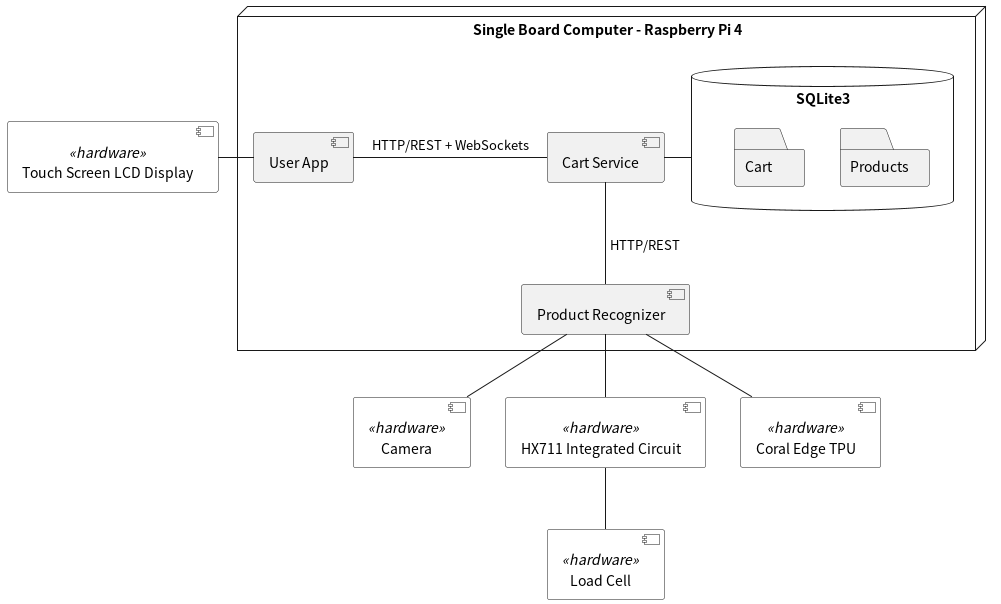
\includegraphics[width=1\textwidth]{./images/zCart.png}
	\caption[High level architecture of zCart]{High level architecture of zCart}
	\fonte{Own work}
	\label{fig:architecture}
\end{figure}


\begin{figure}[H]
	\centering
	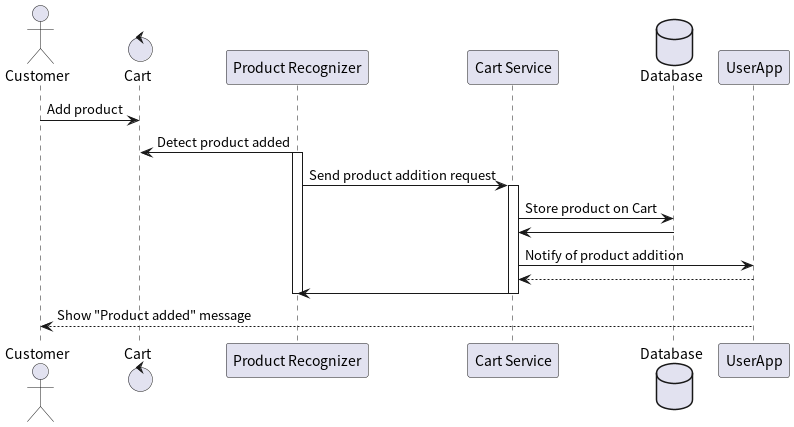
\includegraphics[width=1\textwidth]{./images/E2E.png}
	\caption[End-to-end sequence of interactions]{End-to-end sequence of interactions}
	\fonte{Own work}
	\label{fig:e2eseq}
\end{figure}

\subsection{Architectural Guidelines}
In creating the zCart architecture, the following guidelines were followed:

\begin{itemize}
    \item Create a separate software application for each responsability
    \item Use well defined standards for communication between applications.
    \item All databases should be owned by a single application. 
    \item Any interaction that requires an update to a given database that is
        not owned by an application should be done through an API and not
        directly.
    \item Decouple the user interface from the how the data displayed is stored and transmitted
\end{itemize}

These guideline are based on known best practices from the software development industry including API-first design and segregation of
responsabilities. \cite{Sam2021,Kong2022}

In the sections that follow, each application will be further detailed.

\section{User App}

For developing the User App, we have used web technologies such as HTML, CSS \cite{Duckett2011} and JavaScript \cite{Flanagan2020} through the 
React\footnote{htps://reactjs.org} framework. 

Using web based technologies allows the User App to be display on any device capable of running a web browser and
having mature tooling for development, testing and debugging influenced our decision.

Although developing Linux native graphical applications through toolkits such
as GTK\footnote{https://gtk.org} and Qt\footnote{https://qt.io} might have
yield better performance, our familiarity with web based technologies was a
key deciding factor in favor of using those.

\begin{figure}[H]
	\centering
	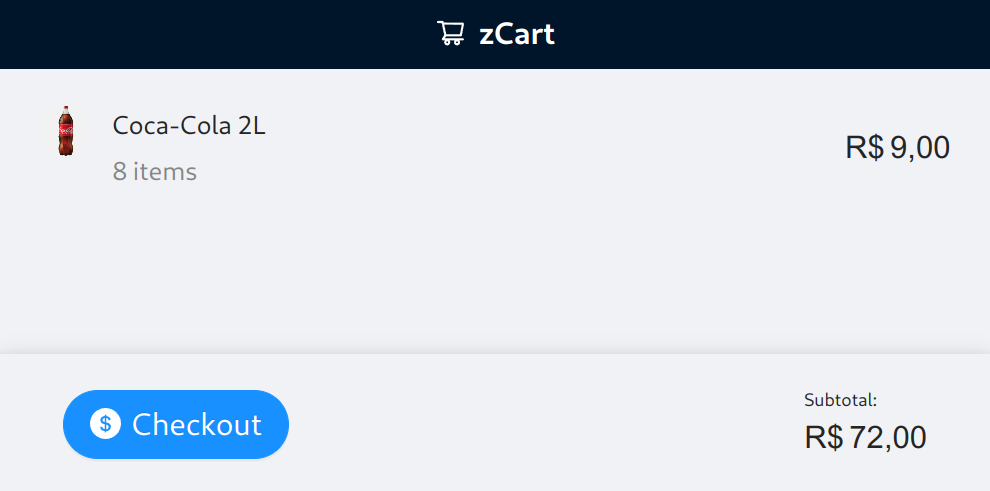
\includegraphics[width=0.8\textwidth]{./images/ui.png}
	\caption[User App Interface display a single product]{User App Interface displaying a single product}
	\fonte{Own work}
	\label{fig:dummy}
\end{figure}

More screenshots are available in Appendix \ref{ap:userapp}.

\begin{figure}[H]
	\centering
	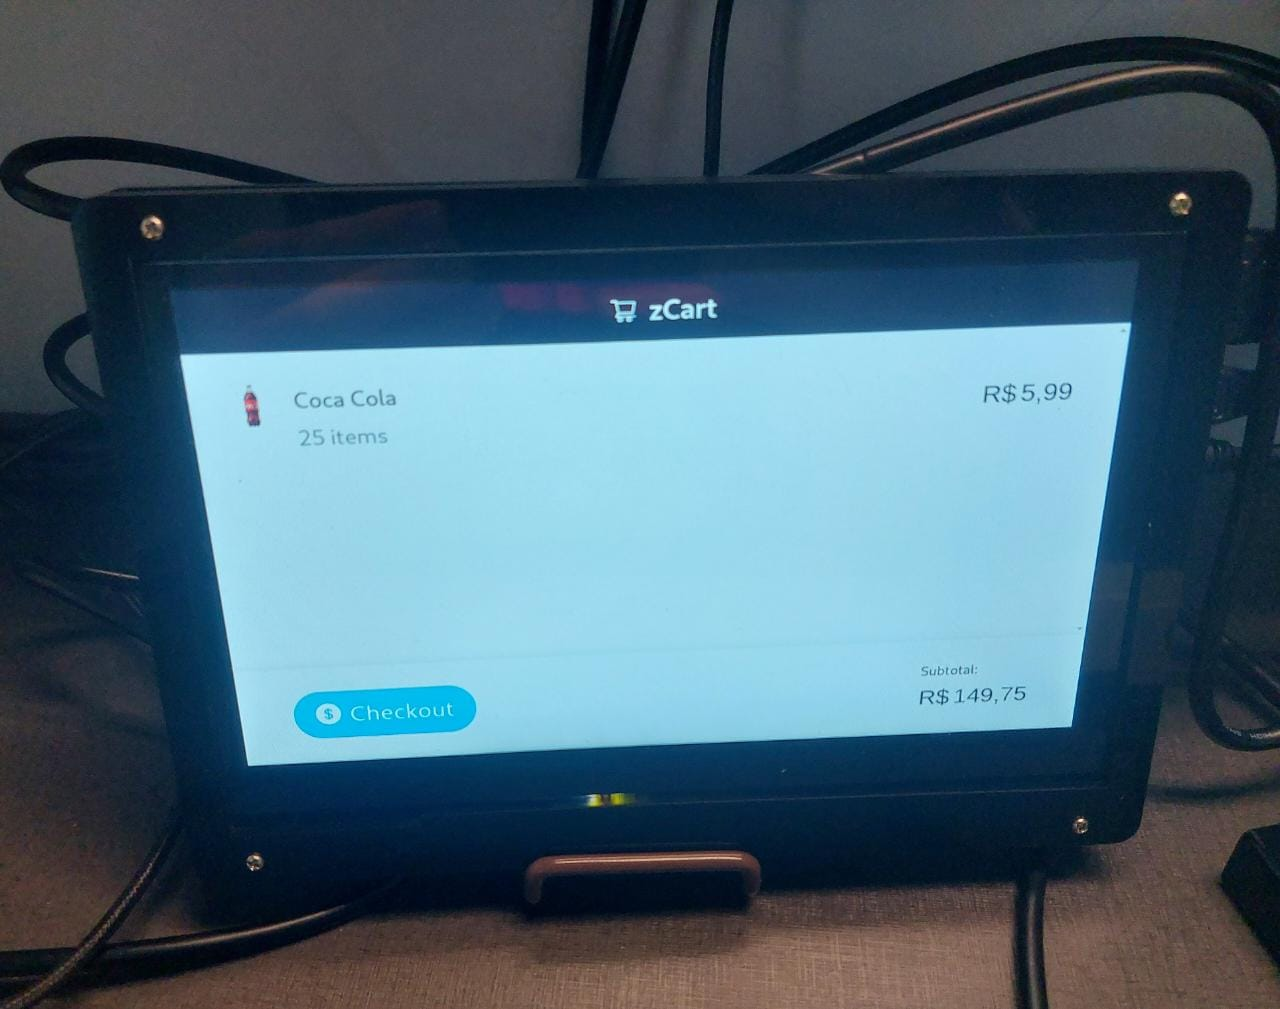
\includegraphics[width=0.8\textwidth]{./images/lcddisplay.jpeg}
	\caption[LCD Display showing the User App]{LCD Display showing the User App}
	\fonte{Own work}
	\label{fig:dummy}
\end{figure}

\section{Product Recognizer}

\subsection{Weight Sensor}

\begin{figure}[H]
	\centering
	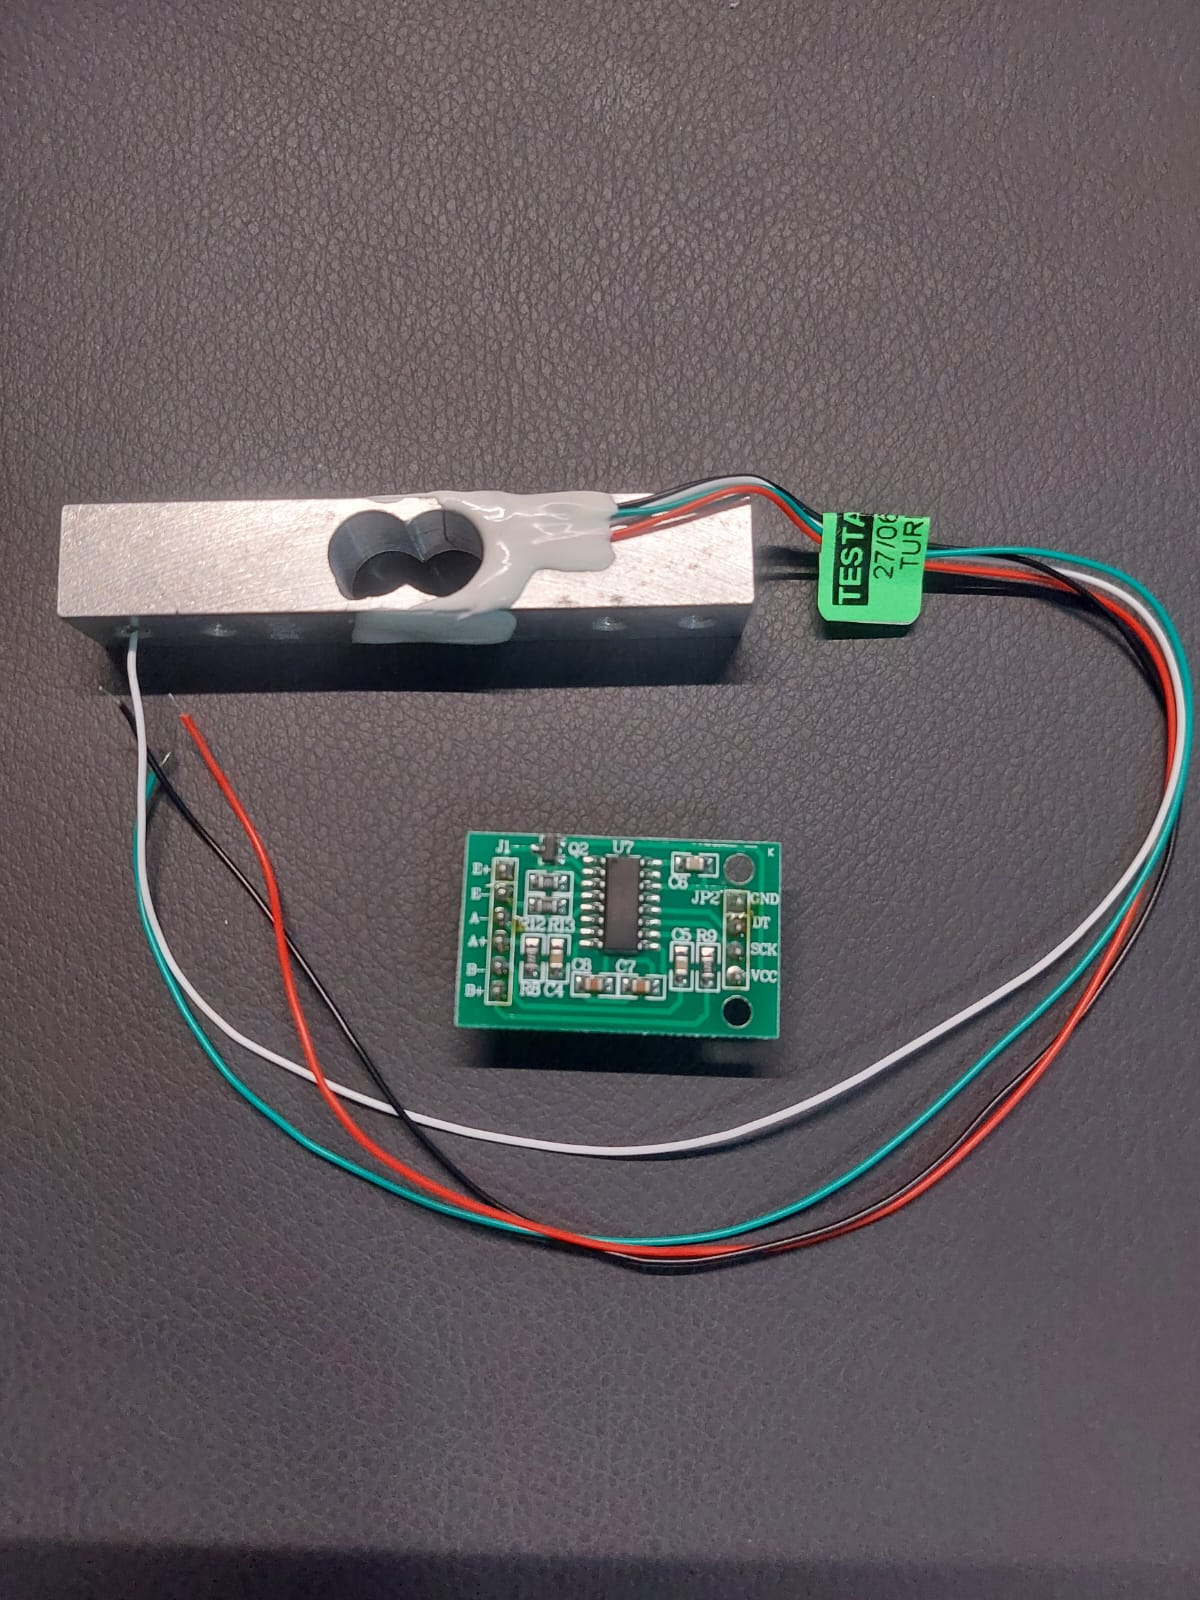
\includegraphics[width=0.5\textwidth]{./images/hx711.jpeg}
	\caption[HX711 breakout board and load cell]{HX711 breakout board and load cell}
	\fonte{Own work}
	\label{fig:dummy}
\end{figure}

\begin{figure}[H]
	\centering
	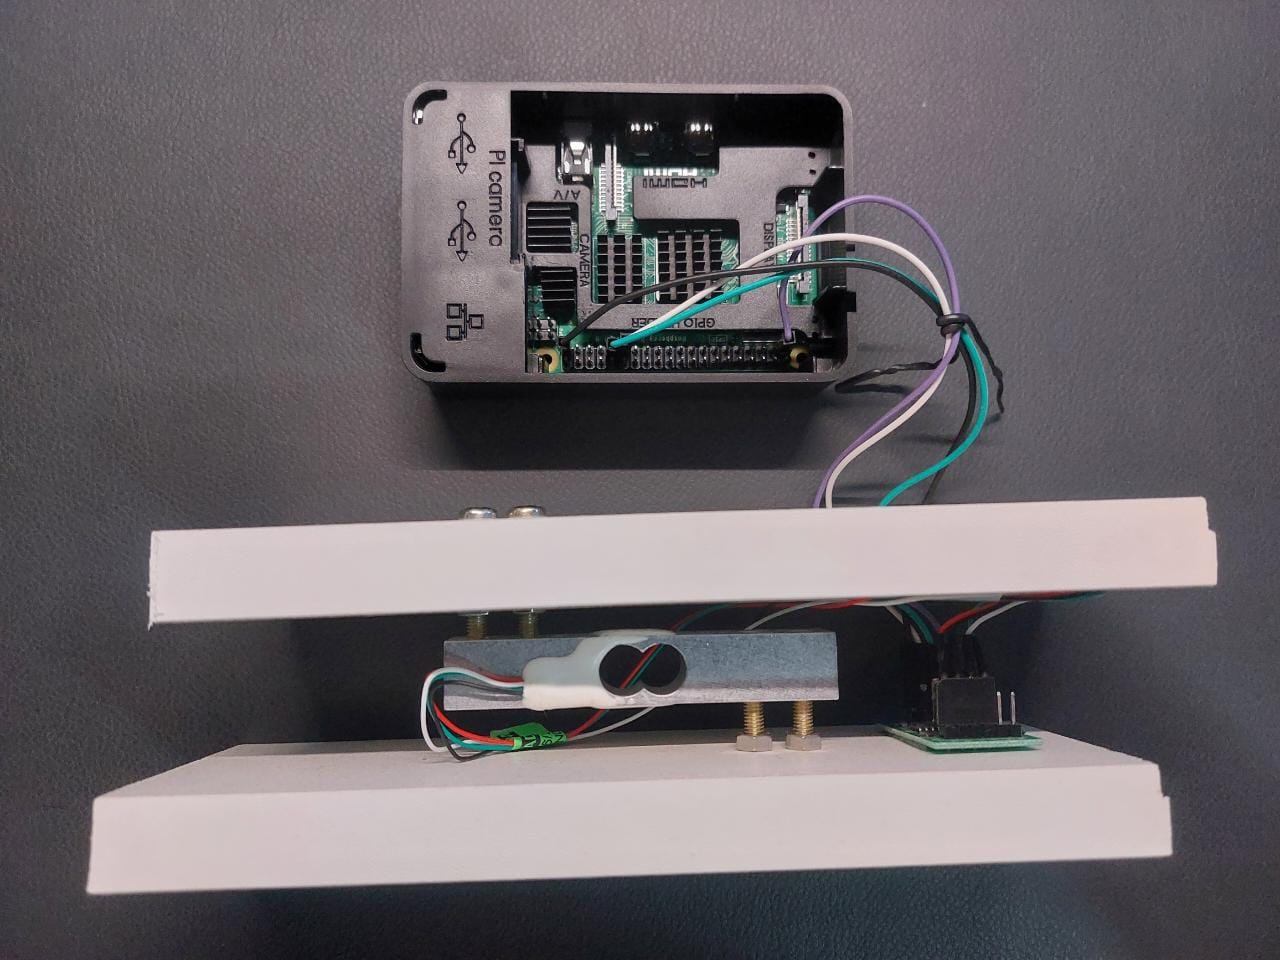
\includegraphics[width=0.8\textwidth]{./images/raspberrypiwithloadcell.jpeg}
	\caption[Scheme used during development, including the Raspberry Pi and load cell assembly]{Scheme used during development, including the Raspberry Pi and load cell assembly}
	\fonte{Own work}
	\label{fig:dummy}
\end{figure}

\begin{figure}[H]
	\centering
	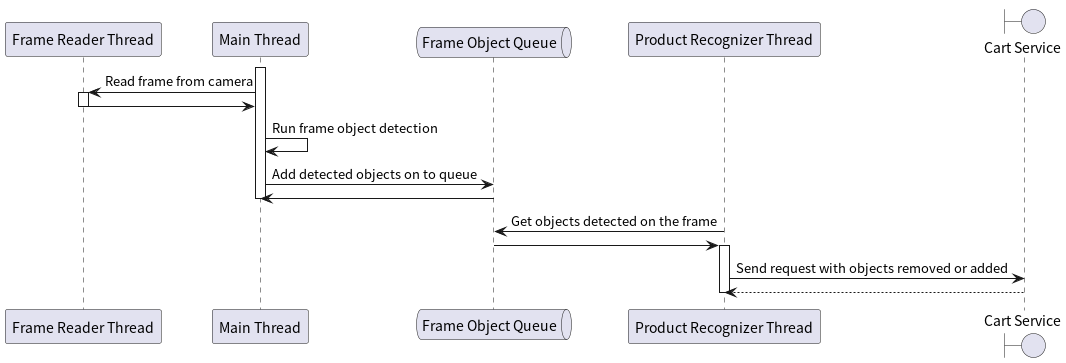
\includegraphics[width=1\textwidth]{./images/Product Recognizer Thread communication.png}
	\caption[Thread communication for the Product Recognizer App]{Thread communication for the Product Recognizer App}
	\fonte{Own work}
	\label{fig:dummy}
\end{figure}

\begin{figure}[H]
	\centering
	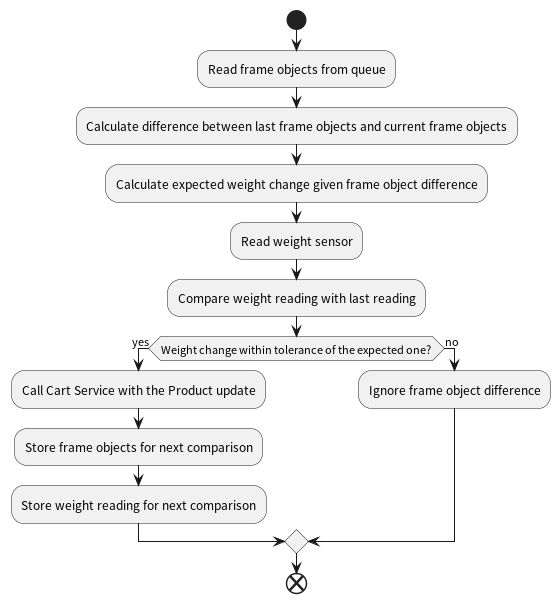
\includegraphics[width=1\textwidth]{./images/Product Recognizer Activity.png}
	\caption[Activity diagram for the Product Recognizer thread]{Activity diagram for the Product Recognizer thread}
	\fonte{Own work}
	\label{fig:dummy}
\end{figure}

\chapter{Conclusions}


%---------- Referencias ----------
\clearpage % this is need for add +1 to pageref of bibstart used in 'ficha catalografica'.
\label{bibstart}
\bibliography{reflatex} % geracao automatica das referencias a partir do arquivo reflatex.bib
\label{bibend}

%---------- Apendices (opcionais) ----------
\apendice
\chapter{User App screenshots}
\label{ap:userapp}

\begin{figure}[H]
	\centering
	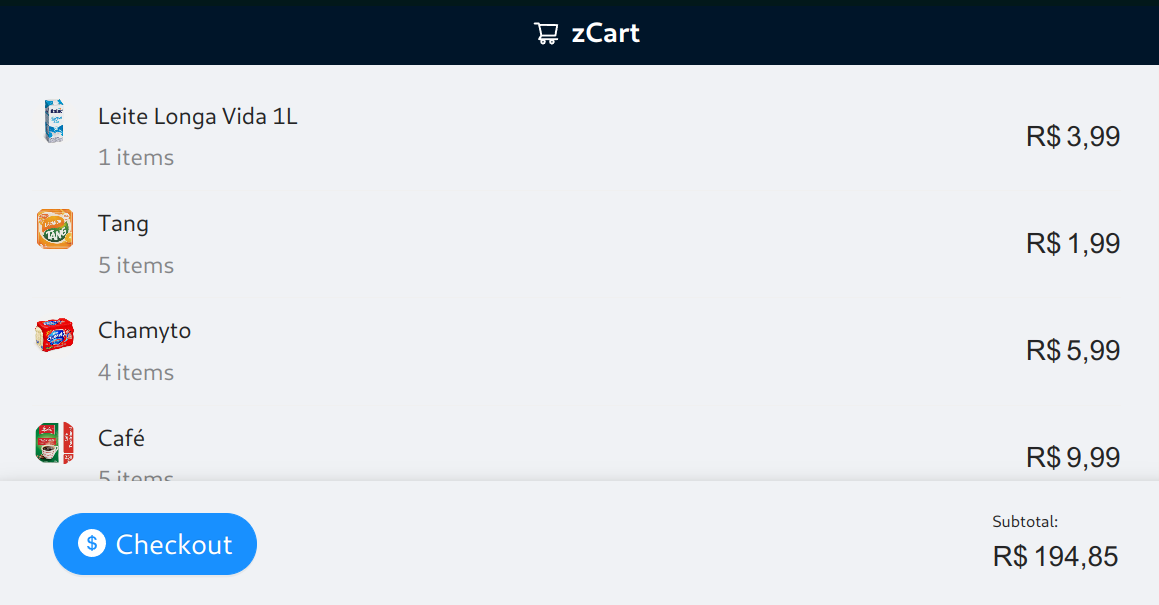
\includegraphics[width=1\textwidth]{./images/userapp.png}
	\caption[]{Product listing and subtotal}
\end{figure}

\begin{figure}[H]
	\centering
	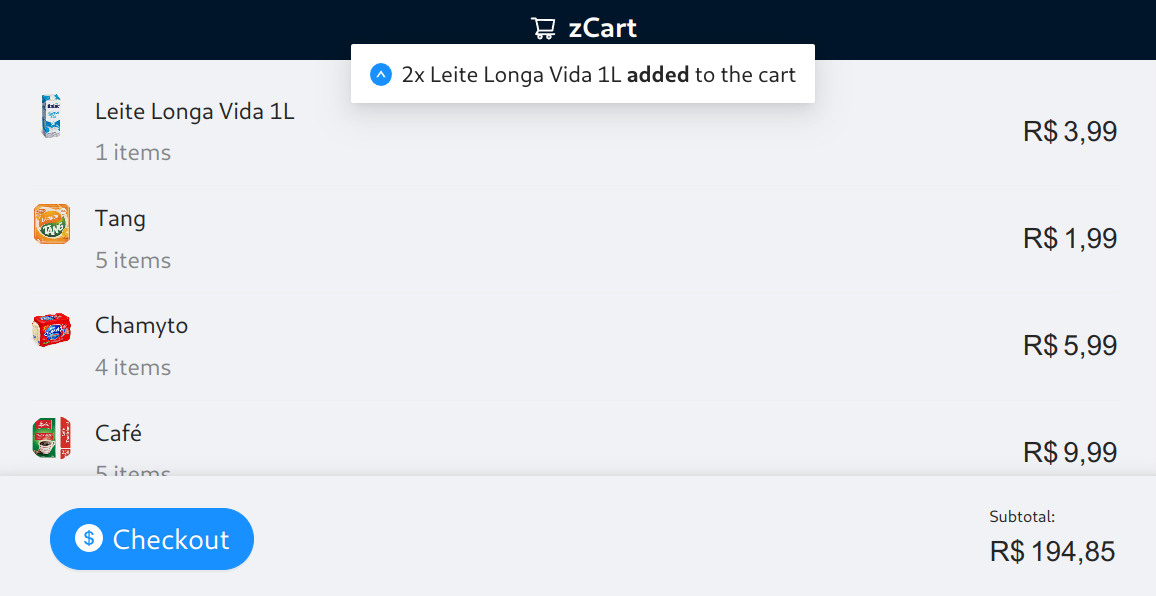
\includegraphics[width=1\textwidth]{./images/userapp2.png}
	\caption[]{Item addition notification}
\end{figure}

\begin{figure}[H]
	\centering
	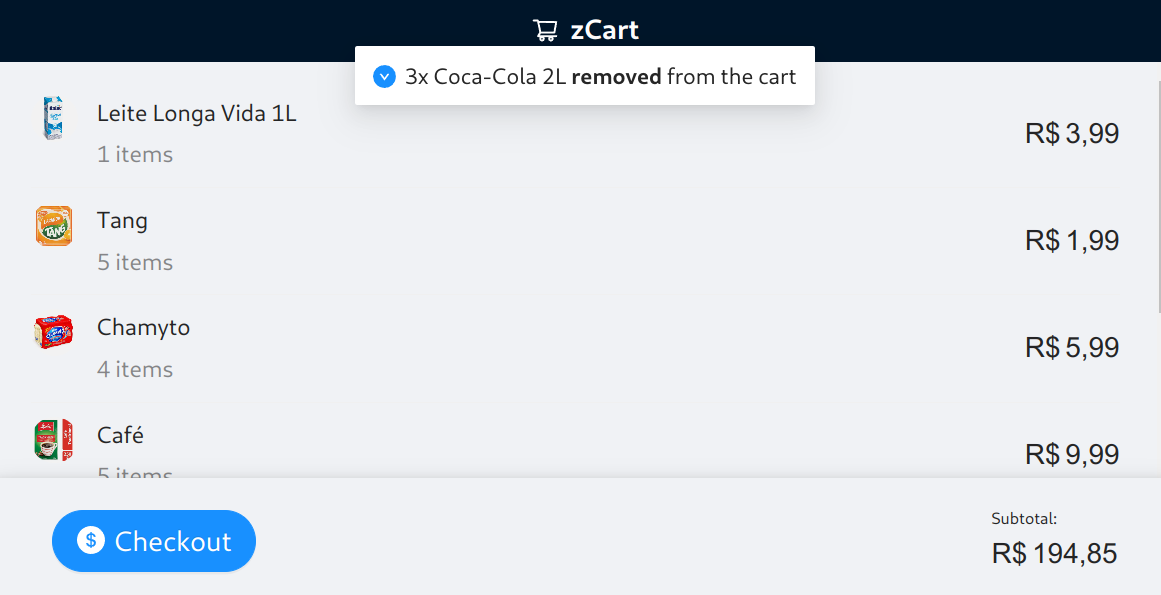
\includegraphics[width=1\textwidth]{./images/userapp3.png}
	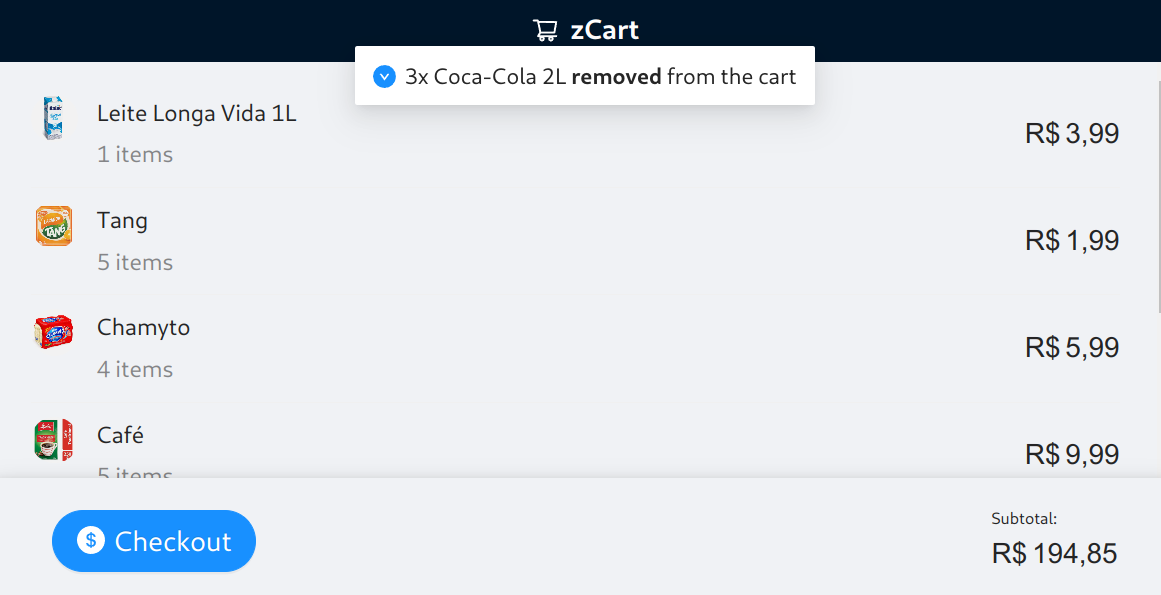
\includegraphics[width=1\textwidth]{./images/userapp3.png}
	\caption[]{Item removal notification}
\end{figure}

\begin{figure}[H]
	\centering
	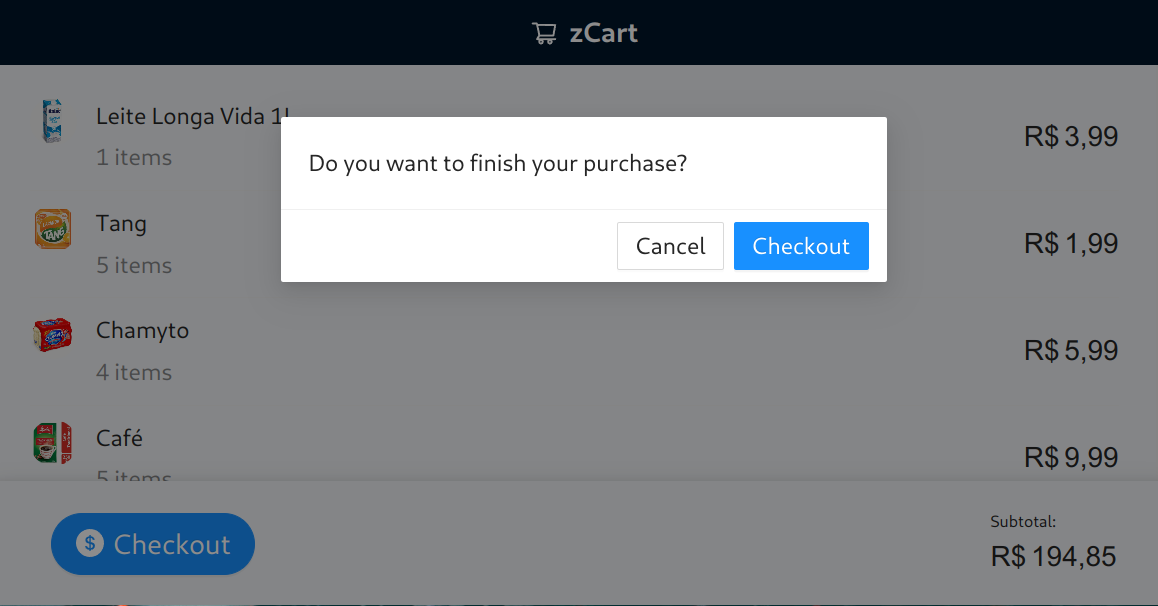
\includegraphics[width=1\textwidth]{./images/userapp4.png}
	\caption[]{Pre-checkout confirmation popup}
\end{figure}

\begin{figure}[H]
	\centering
	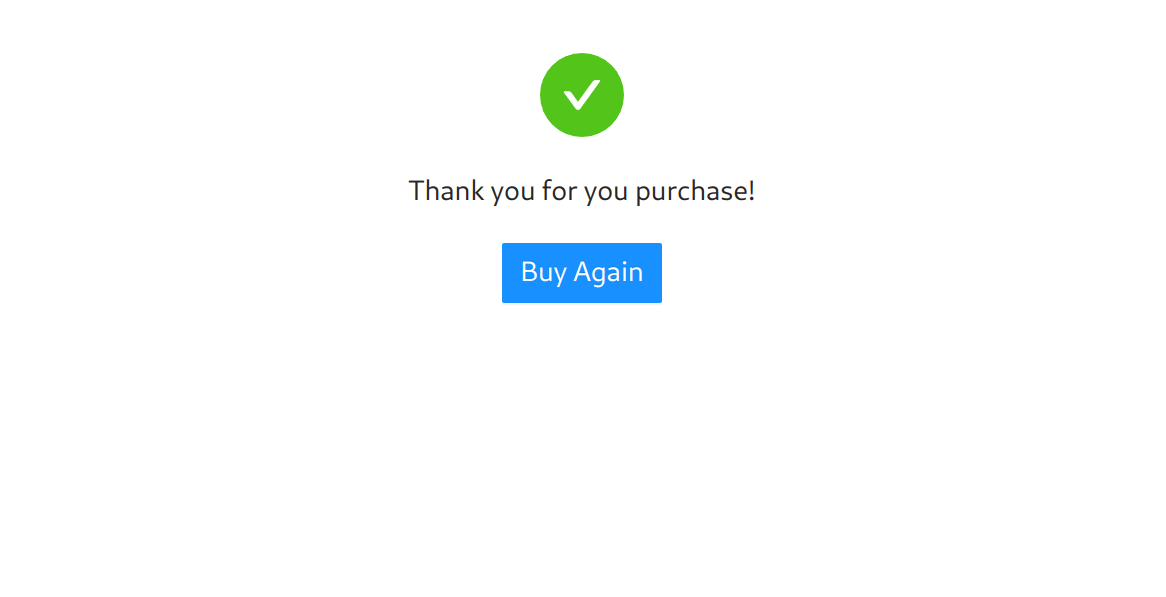
\includegraphics[width=1\textwidth]{./images/userapp5.png}
	\caption[]{Post checkout screen}
\end{figure}

\anexo
\chapter{Nome do Anexo}

Use o comando {\ttfamily \textbackslash anexo} e depois comandos {\ttfamily \textbackslash chapter\{\}}
para gerar titulos de anexos.
\end{document}
